\documentclass[12pt,a4paper]{article}
\usepackage{amsmath}
\usepackage{amssymb}  % Provides \mathbb and other symbols
\usepackage{graphicx}
\usepackage{subcaption}
\usepackage{enumitem}
\usepackage{listings}
\usepackage{hyperref}
\usepackage{ulem}
\usepackage{xcolor}
\usepackage{amsthm}
\usepackage{tcolorbox}     % For colored boxes
\usepackage[table]{xcolor} % For coloring table cells
\usepackage{array}         % For better table alignment
\usepackage{mdframed}
\usepackage{cancel}
\usepackage[margin=2.5cm]{geometry}
\usepackage{lmodern}
\setlength{\parindent}{0pt}
\setlength{\parskip}{0.8em}
\newcommand{\answer}{\vspace{3\baselineskip}\textbf{ANSWER:}}
\newcommand{\question}[2]{\textbf{Question #1}\quad #2}

\begin{document}

\begin{titlepage}
\centering
\vspace*{\fill} % Adds vertical space to center the title block vertically

{\Huge Complex Analysis} \\[0.5cm] % Title 2
{\Huge Home Work 1}\\[1.5cm] % Title 3
{\Large Student: Mark Roberts [26-712-224]}\\[0.5cm] % Student ID
{\Large \today} % Date, \today adds today's date

\vspace*{\fill}
\end{titlepage}
\newpage

\question{1.1}{
\begin{enumerate}
\item[(a)] Find the modulus and the principal branch of argument of the following complex numbers. Hence write them in polar form.

\begin{enumerate}
\item[(i)] $1+i$
\item[(ii)] $6+2\sqrt{3}\,i$
\item[(iii)] $\dfrac{\sqrt{2}}{1-i}$
\end{enumerate}

\item[(b)] Write the following complex numbers in the form $a+bi$:
\begin{enumerate}
\item[(i)] $2e^{3\pi i/4}$
\item[(ii)] $e^{7\pi i/6}$
\item[(iii)] $\dfrac{1+i}{i}+\dfrac{i}{1-i}$
\end{enumerate}

\item[(c)] Write the following complex numbers in the form $a+bi$, and in polar form:
\begin{enumerate}
\item[(i)] $\dfrac{1+i}{\sqrt{3}-3i}$
\item[(ii)] $(1-i)^3$
\item[(iii)] $\left(\sqrt{2+\sqrt{2}}+\sqrt{2-\sqrt{2}}\,i\right)^2$
\end{enumerate}

Using your answer to (iii), deduce the value of $\cos\dfrac{\pi}{8}$.
\end{enumerate}
}

\answer

(a.i) $|1 + i| = \sqrt{1^2 + 1^2} = \sqrt{2}$ \\
(a.ii) $\left|6 + 2\sqrt{3} i\right| = \sqrt{6^2 + (2\sqrt{3})^2} = \sqrt{36+12} = 4\sqrt{3}$ \\
(a.iii) $\left|\frac{\sqrt{2}}{1-i}\right| = \frac{\sqrt{2}}{|1-i|} = \frac{\sqrt{2}}{\sqrt{1^2 + (-1)^2}} = 1$ \\
(b.i) $2e^{3\pi i/4} = 2(\cos{(3\pi/4)} + i \sin{(3\pi/4)}) = 2(\frac{1}{\sqrt{2}})(-1 + i) = -\sqrt{2} + \sqrt{2} i$ \\
(b.ii) $e^{7\pi i/6} = (\cos{(7\pi/6)} + i \sin{(7\pi/6)}) = (-\frac{\sqrt{3}}{2} - \frac{1}{2} i)$ \\
(b.iii)
\begin{align*}
  \dfrac{1+i}{i}+\dfrac{i}{1-i} &= \left(\dfrac{-i}{-i}\right) \dfrac{1+i}{i} + \left(\dfrac{1+i}{1+i}\right) \dfrac{i}{1-i} \\
  &= (1-i) + \dfrac{-1+i}{2} \\
  &= \dfrac{1-i}{2}
\end{align*}
\newpage
(c.i)
\begin{align*}
\dfrac{1+i}{\sqrt{3}-3i}
&= \left(\dfrac{\sqrt{3}+3i}{\sqrt{3}+3i}\right)\left(\dfrac{1+i}{\sqrt{3}-3i}\right) \\
&= \dfrac{(\sqrt{3}+3i)(1+i)}{(\sqrt{3})^2+3^2} \\
&= \dfrac{(\sqrt{3}-3)+i(\sqrt{3}+3)}{12} \\
&= \dfrac{\sqrt{3}-3}{12}+i\dfrac{\sqrt{3}+3}{12}
\end{align*}

(c.ii)
\begin{align*}
(1-i)^3 &= (1-i)^2(1-i) \\
&= -2i(1-i) \\
&= -2-2i
\end{align*}

(c.iii)
\begin{align*}
\left[\sqrt{2+\sqrt{2}}+\sqrt{2-\sqrt{2}}\,i\right]^2
&= (2+\sqrt{2})+2\left(\sqrt{2+\sqrt{2}}\right)\left(\sqrt{2-\sqrt{2}}\right)i-(2-\sqrt{2}) \\
&= 2\sqrt{2}+2\sqrt{4-2}\,i \\
&= 2\sqrt{2}+2\sqrt{2}\,i
\end{align*}

\newpage

\newpage

\question{1.2}{

\begin{enumerate}
\item[(a)] What do the following subsets represent geometrically? Draw a sketch of each one in the complex plane.

\begin{enumerate}
\item[(i)] $|z+1+i|=1$
\item[(ii)] $1<\operatorname{Re} z\leq 2$
\item[(iii)] $|z-2|<3$ and $|\operatorname{Im} z|>1$
\item[(iv)] $\operatorname{Im} z^2\geq 0$
\end{enumerate}

\item[(b)] Which of the above sets are

\begin{enumerate}
\item[(i)] Open?
\item[(ii)] Closed?
\end{enumerate}
\end{enumerate}

}

\answer

(a.i) $|z+1+i|=1 \Rightarrow |z-(-1-i)|=1$
This represents a circle with centre $(-1-i)$ and radius 3. \\
\\
(a.ii)
$1<\operatorname{Re}(z)\leq 2$ represents a vertical strip in the Argand diagram.

The region in question is shown shaded.

$x=1$ \textbf{is not} in the region.

$x=2$ \textbf{is} in the region.

\begin{center}
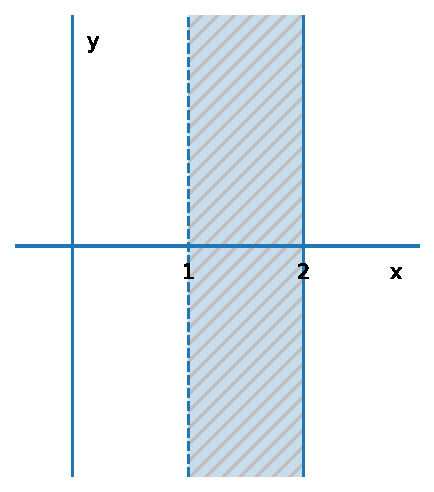
\includegraphics[width=0.38\textwidth]{Diagrams/CA_HW_1_Q1_2_aii.pdf}
\end{center}

(a.iii)
$|z-2|<3$ represents the inside of a circle centred at $2+0i$ with radius 3.

$|\operatorname{Im}(z)|>1$ represents the section of the Argand diagram for which $y>1$.

Any $z\in\mathbb{C}$ that satisfies both conditions will be in the inside of the circle (centred on $2+0i$, with radius 3) and lies above the line $y=1$.

The shaded region in the diagram is the required region.

\begin{center}
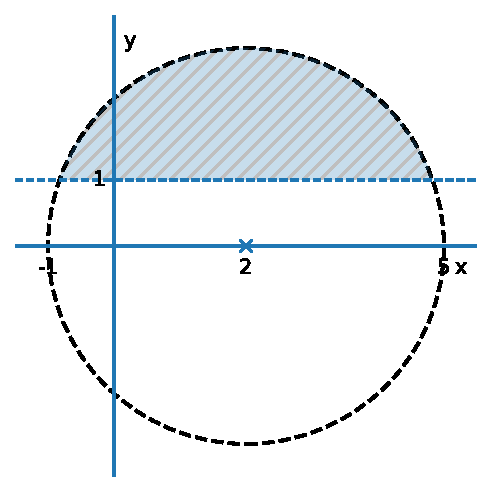
\includegraphics[width=0.45\textwidth]{Diagrams/CA_HW_1_Q1_2_aiii.pdf}
\end{center}

(a.iv)
$\operatorname{Im} z^2\geq 0$.  Let $z=x+yi \Rightarrow z^2=x^2-y^2+2xyi$
$\Rightarrow \operatorname{Im}(z^2)=2xy$. \\
\\
Now $2xy \ge 0$ is given by the 2 quadrants shown below.

\begin{center}
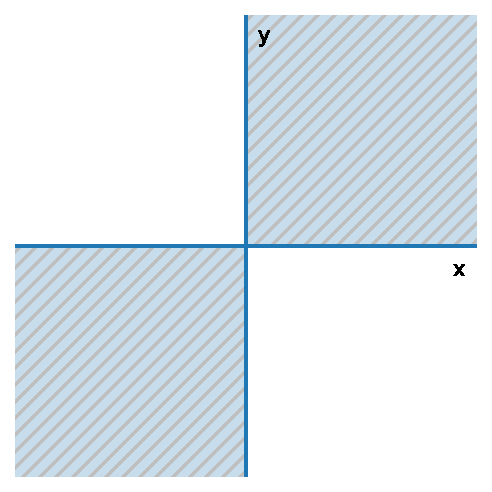
\includegraphics[width=0.38\textwidth]{Diagrams/CA_HW_1_Q1_2_aiv.pdf}
\end{center}

\newpage
(b)(i) The boundary of a circle is a \textbf{closed} set. \\
\\
(ii) The boundary is open on one side $(x=1)$ \& closed on the other $(x=2)$.
So the region is \textbf{neither open nor closed}. \\
\\
(iii) The two sets in question are both open.  This $\Rightarrow$ their intersection will also be an \textbf{open} set.\\
\\
(iv) The $x=0$ \& $y=0$ are included in the region (since the two regions contain all their limit pts) $\Rightarrow$ region 
is a \textbf{closed} set.

\newpage

\question{1.3}{Find all roots in $\mathbb{C}$ of the following equations (you may express your answer in either $a+bi$ or polar form, whichever you prefer):

\begin{enumerate}
\item[(i)] $z^3+1=0$
\item[(ii)] $1+z+z^2=0$ \qquad \emph{*Hint: First try expanding $(z-1)(1+z+z^2)$.*}
\item[(iii)] $1-z^2+z^4=0$
\end{enumerate}

}

\answer \\
(i)\quad $z^3+1=0$.  Let $z=re^{i\theta}$.  Then we get:
\[
(re^{i\theta})^3+1=0
\]

\[
\Rightarrow r^3e^{3i\theta}=-1 \tag{A}
\]

As $r \ge 0 \Rightarrow r=1$.  Using (A) we can determine the $\theta$ values as:

\[
\theta_n=\frac{\pi(2n+1)}{3},\qquad n \in \{0,1,2\}
\]

From which:

\[
\begin{aligned}
\theta_0 &= \frac{\pi}{3},\qquad
\theta_1 &= \pi,\qquad
\theta_2 &= \frac{5\pi}{3}
\end{aligned}
\]

We can now calculate the $z_n$:
\[
z_0=e^{i\pi/3}
=\frac12+\frac{\sqrt3}{2}i
\]

\[
z_1=e^{i\pi}=-1
\]

\[
z_2=e^{i5\pi/3}
=\frac12-\frac{\sqrt3}{2}i
\]

(ii)\quad Clearly $1+z+z^2=0$ is not satisfied by $z=1$.\\
Now:

\[
(z-1)(1+z+z^2)=z^3-1 \tag{B}
\]

Now the solutions of (B) are just the solutions of $1+z+z^2 = 0$ and $z=1$ and
follow the same sort of pattern as (i) above, but in this case: $z^3=1=e^{i0}$.\\
These solutions are:
\[
\theta_n=\frac{2n\pi + 0}{3},\qquad n \in \{0,1,2\}
\]
We can ignore $\theta_0 = 0$, as this is the $z=1$ solution.  The solutions to $1+z+z^2=0$
are found when $n=1,2$:

\[
\begin{aligned}
z_1=e^{i2\pi/3} &= -\frac12+\frac{\sqrt3}{2}i \\
z_2=e^{i4\pi/3} &= -\frac12-\frac{\sqrt3}{2}i
\end{aligned}
\]

(iii)\quad $1 - z^2 + z^4 = 0$ can be simplified by replacing $y=-z^2$ in which case we 
would then have the equivalent equation:
\[
1 + y + y^2 = 0 \tag{C}
\]
We have already solved this equation in (ii) above.  The solutions being: $y_1 = -z_1^2 =e^{i2\pi/3}$
and $y_2 = -z_2^2 =e^{i4\pi/3}$. Or, equivalently: $z_1^2 = e^{i5\pi/3}$ and 
$z_2^2 =e^{i7\pi/3}$.\\
\\
Each solution has two seperate solutions for $z$ - so we have a total of 4 solution:
\[
\begin{aligned}
z_{11} &= e^{i5\pi/6} &= -\frac{\sqrt3}{2} + \frac{1}{2}i \\
z_{12} &= -e^{i5\pi/6} &= \frac{\sqrt3}{2} - \frac{1}{2}i  \\
z_{21} &= e^{i7\pi/6} &= -\frac{\sqrt3}{2} - \frac{1}{2}i \\
z_{22} &= -e^{i7\pi/6} &= +\frac{\sqrt3}{2} + \frac{1}{2}i
\end{aligned}
\]

\newpage

\question{1.4}{For each of the following, either find the limit or prove that it does not exist, as appropriate.

\begin{enumerate}
\item[(i)] $\displaystyle \lim_{z\to 3+4i}(z-7i)^2$
\item[(ii)] $\displaystyle \lim_{z\to 0}\frac{\operatorname{Re}z+\operatorname{Im}z}{z}$
\item[(iii)] $\displaystyle \lim_{z\to 2i}\frac{z^2+4}{z-2i}$
\end{enumerate}
}

\answer\\
(i)

As $(z-7i)^2$ is a continuous function on $\mathbb{C}$, we can replace $z$ by $3+4i$:

\[
\lim_{z\to 3+4i}(z-7i)^2
=
(3+4i-7i)^2
=
(3-3i)^2
=
-18i
\]

(ii)

\[
\frac{\operatorname{Re}(z)+\operatorname{Im}(z)}{z}
=
\frac{x + y}{x + iy}
\]
Hence:
\[
\lim_{z\to 0} \frac{\operatorname{Re}(z)+\operatorname{Im}(z)}{z}
=
\lim_{z\to 0} \frac{x + y}{x + iy}
\]

But this has no limit, since along the real line the limit is 1 and along the imaginary line th limit is i.\\
\\
(iii)

\[
z^2+4=(z+2i)(z-2i)
\]

\[
\Rightarrow
\lim_{z\to 2i}\frac{z^2+4}{z-2i}
=
\lim_{z\to 2i}(z+2i)
=
4i
\]

\newpage

\question{1.5}{For each of the following functions, write the real and imaginary parts as functions of $(x,y)$, where $z=x+iy$.

\begin{enumerate}
\item[(i)] $z^3+2z+1$
\item[(ii)] $z+z^{-1}$ (for $z\neq 0$)
\item[(iii)] $\dfrac{1}{1-z}$ (for $z\neq 1$)
\end{enumerate}
}

\answer \\
(i)
\[
\begin{aligned}
z^3 &= (x+iy)^3=(x+iy)(x^2-y^2+2xyi) \\
    &= x(x^2-y^2)-2xy^2+iy(x^2-y^2)+2x^2yi \\
    &= x(x^2-3y^2)+iy(3x^2-y^2)
\end{aligned}
\]

\[
\Rightarrow z^3+2z+1
=
\left[x(x^2-3y^2+2)+1\right]
+i\left[y(3x^2-y^2+2)\right]
\]
From which we can determine the real and immaginary functions as:
\[
\begin{aligned}
u(x,y) &= x(x^2-3y^2+2)+1 \\
v(x,y) &= y(3x^2-y^2+2)
\end{aligned}
\]
Where: $u(x,y)$ is the real function and $v(x,y)$ is the imaginary function.\\
\\
(ii) For $z \ne 0$ we have:
\[
\begin{aligned}
z + \frac{1}{z} &= (x+iy) + \frac{1}{x+iy} \\
 &= (x + iy) + \frac{x-iy}{x-iy}\frac{1}{x+iy} \\
 &= (x + iy) +\frac{x-iy}{x^2+y^2} \\
 &= (x + \frac{x}{x^2+y^2}) + i (y - \frac{y}{x^2+y^2}) \\
 &= x(1 + \frac{1}{x^2+y^2}) + i y(1 - \frac{1}{x^2+y^2})
 \end{aligned}
\]
From which we determine that:
\[
u(x,y)=x(1 + \frac{1}{x^2+y^2})
\qquad
v(x,y)=y(1 - \frac{1}{x^2+y^2})
\]

are the real \& complex functions respectively.

\newpage
(iii) For $z \ne 1$ we have:
\[
\begin{aligned}
\frac{1}{1-z} &= \frac{1}{(1-x) - iy} \\
    &= \frac{1}{(1-x) - iy} \frac{(1-x) + i y}{(1-x) + i y} \\
    &= \frac{(1-x) + i y}{(1-x)^2 + y^2}
\end{aligned}
\]
From which we determine that:
\[
u(x,y)=\frac{(1-x)}{(1-x)^2 + y^2}
\qquad
v(x,y)= \frac{y}{(1-x)^2 + y^2}
\]


\newpage

\question{1.6}{Prove that, for all $z,w\in\mathbb{C}$,

\[
|z+iw|^2+|w+iz|^2=2\bigl(|z|^2+|w|^2\bigr).
\]

\emph{*Extra$^*$: Can you see a geometric interpretation of this identity?*}

}

\answer \\
\[
|z+iw|^2=(z+iw)(\bar{z}-i\bar{w})
\]

\[
=|z|^2+|w|^2+iw\bar{z}-iz\bar{w}
\]

\[
|w+iz|^2=(w+iz)(\bar{w}-i\bar{z})
\]
\[
=|w|^2+|z|^2+iz\bar{w}-iw\bar{z}
\]
Note that the terms in the expansion that contain i have opposite signs - so summing 
the two terms will cause them to cancel:

\[
\Rightarrow |z+iw|^2+|w+iz|^2
=2|z|^2+2|w|^2
\]

\[
=2\left(|z|^2+|w|^2\right)
\]
\qed
\\
\\
This formula is nothing more that the parallelogram law.
\begin{center}
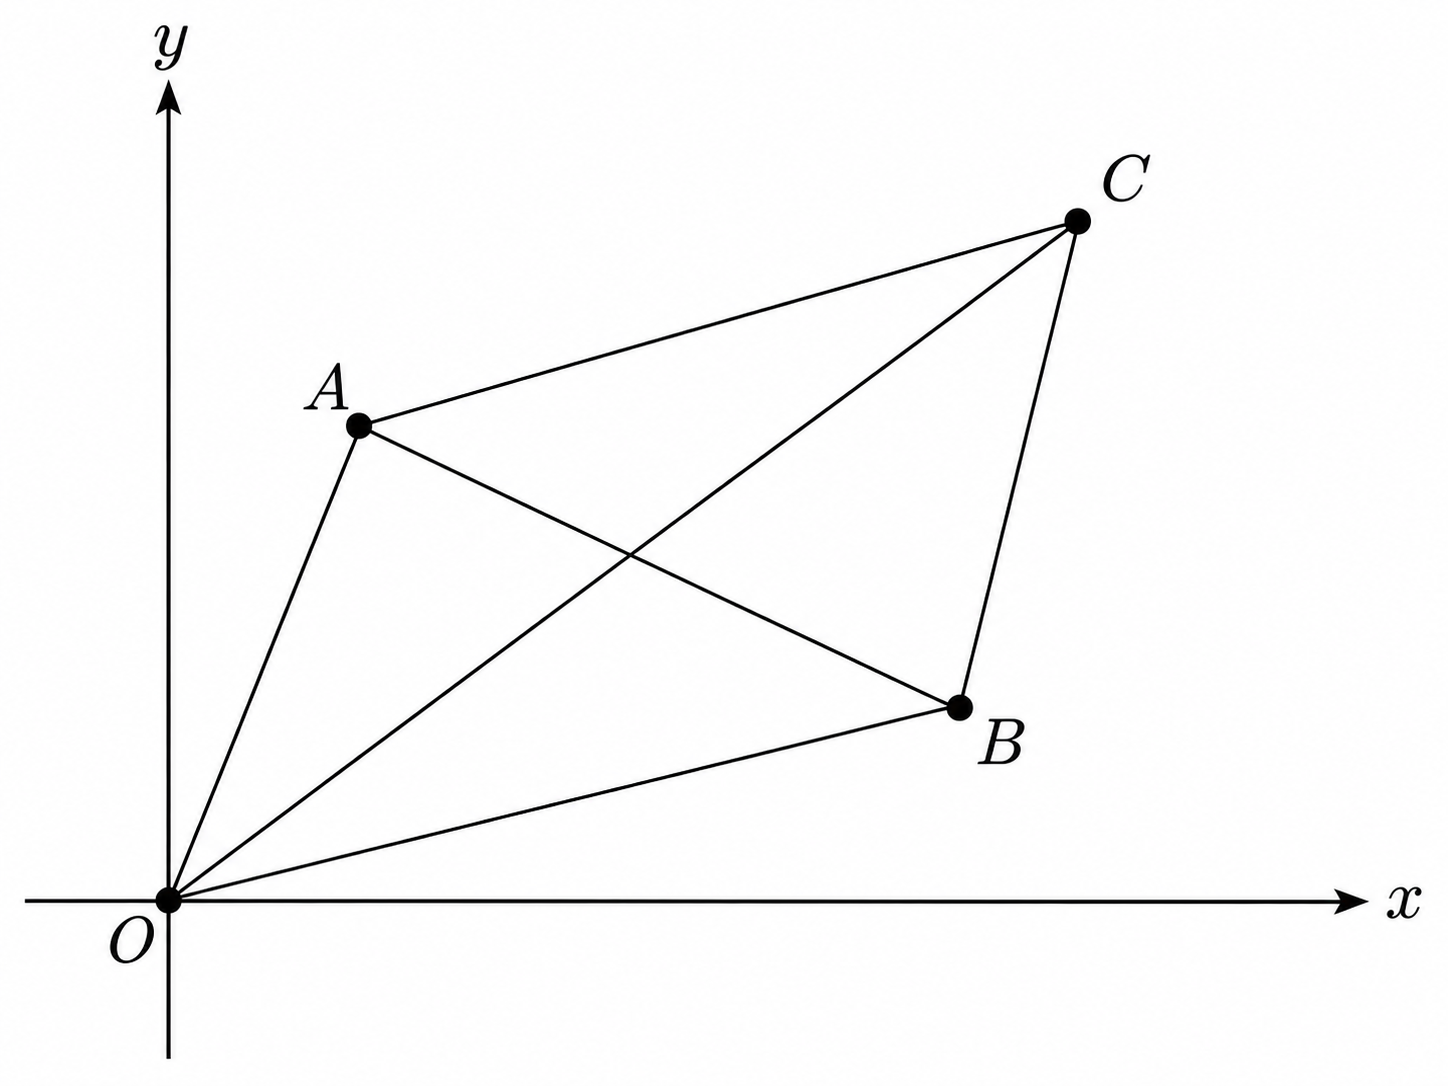
\includegraphics[width=0.45\textwidth]{Diagrams/CA_HW_1_Q1_6.png}
\end{center}
This law states that for a parallelogram (shown above) we have:
\[
\begin{aligned}
2(|OA|^2 + |OB|^2) = |AB|^2 + |OC|^2
\end{aligned} \tag{1.6A}
\]

Take $z = OB$ and $iw = OA$ and noting that $|iw|=|w|$.  Then (1.6A) becomes:
\[
\begin{aligned}
2(|z|^2 + |w|^2) = |z+iw|^2 + |z-iw|^2
\end{aligned}  \tag{1.6B}
\]
This is already near the formula we want [i.e. $|z+iw|^2+|w+iz|^2=2\bigl(|z|^2+|w|^2\bigr)$]; we only
need to show that $|z-iw|=|w+iz|$.  Now:
\[
\begin{aligned}
w+iz &= i(z-iw) \\
\implies |w+iz| &= |i(z-iw)| \\
&= |z-iw|
\end{aligned}
\]

\qed

\newpage

\question{1.7}{Show that, for all $z,w\in\mathbb{C}$ such that $|z|<1$ and $|w|<1$,

\[
\left|\frac{z-w}{1-\overline{z}w}\right|<1.
\]

Now assume that $z,w\in\mathbb{C}$ with $1-\overline{z}w\neq 0$ (but not necessarily that $|z|<1$ and $|w|<1$). For which $z,w$ do we have

\[
\left|\frac{z-w}{1-\overline{z}w}\right|=1?
\]
}

\answer\\

$z,w\in\mathbb{C}$ and $|z|<1$ \& $|w|<1$.  Now:

\[
\left|\frac{z-w}{1-\overline{z}w}\right|<1
\]

\[
\Leftrightarrow |z-w|<|1-\overline{z}w|
\]

\[
\Leftrightarrow |z-w|^2<|1-\overline{z}w|^2
\]

\[
\Leftrightarrow (z-w)(\overline{z}-\overline{w})
<
(1-\overline{z}w)(1-z\overline{w})
\]

\[
\Leftrightarrow
|z|^2-z\overline{w}-\overline{z}w+|w|^2
<
1-z\overline{w}-\overline{z}w+|z|^2|w|^2
\]

\[
\Leftrightarrow
0 < 1-|z|^2-|w|^2+|z|^2|w|^2
\]

\[
\Leftrightarrow
0<(1-|w|^2)(1-|z|^2) \quad \quad \quad \quad \text{(***)}
\]

As $|z|<1$ \& $|w|<1$

\[
(1-|w|^2)>0
\quad \&
\quad
(1-|z|^2)>0.
\]

And hence equation (***) holds.  Consequently:

\[
\Rightarrow
\left|\frac{z-w}{1-\overline{z}w}\right|<1.
\]

For equality to hold

\[
\left|\frac{z-w}{1-\overline{z}w}\right|=1
\Leftrightarrow
|z-w|^2=|1-\overline{z}w|^2
\]

\[
\Leftrightarrow
|w|^2+|z|^2=1+|z|^2|w|^2
\]

\[
\Leftrightarrow
0=1-|w|^2-|z|^2+|z|^2|w|^2
\]

\[
=(1-|w|^2)(1-|z|^2)
\]

\[
\Rightarrow |w|=1 \quad \text{or} \quad |z|=1.
\]
We need to qualify this last result as we must also have that $1 - \overline{z}w \ne 0$.
So we must exclude the condition $z=w$.

\newpage

\question{1.8}{Prove Cantor's Intersection Theorem (Theorem 1.44 in the Lecture Notes).}\\
\\
\textbf{Theorem 1.44 (Cantor's Intersection Theorem).}
\textit{Let $K\subset\mathbb{C}$ be a compact set, and let
$\{C_n\}_{n=1}^{\infty}$ be non-empty closed sets with
$C_n\subset K$ for all $n\in\mathbb{N}$, that are nested such that
$C_{n+1}\subset C_n$ for all $n\in\mathbb{N}$.
Then
\[
\bigcap_{n=1}^{\infty} C_n \neq \varnothing.
\]
}

\answer\\
From the definition of $\{C_n\}$ in the theorem it is clear that

\[
C_n=\bigcap_{i=1}^{n} C_i \qquad (\neq \emptyset)\qquad \forall n\in\mathbb N
\]
As $K$ is compact we know that it is sequentially compact.\\
\\
Construct a Sequence $\{z_n\}$ by selecting each $z_n$ from $C_n$ $(n=1,2,\ldots)$.  Then, as $\{z_n\}$ is a sequence in the sequentially compact set $K$:

\[
\Rightarrow \exists \{z_{n_k}\}\subset\{z_n\} \text{ that converges to } z\in K
\]

But $\{z_{n_k}\}$ is also a convergent subsequence in each $C_n$ and, as $C_n$ is closed, $z\in C_n$. This is true for every $C_n,\ n\in\mathbb N$. Hence

\[
z\in\bigcap_{i=1}^{\infty} C_n
\qquad\Rightarrow\qquad
\bigcap_{i=1}^{\infty} C_n\neq\emptyset
\]
\qed

\end{document}
